\chapter{Результаты} \label{ch3}
\par Данная глава посвящена анализу результатов экспериментов по денойзингу с использованием различных методов, а также автоматической сегментации трёхмерных сфер. Особое внимание уделяется результатам интеграции и внедрения реализованных методов в онлайн-сервис.
\section{Результаты денойзинга}
\par В этом разделе особое внимание уделяется процессу обучения модели Noise2Noise, а также экспериментам, проводившимся на реальных и синтетических снимках различными методами денойзинга.
\subsection{Используемые метрики}
\par Для оценки качества работы методов денойзинга использовались следующие метрики \cite[с. 6-8]{zhang2019poissongaussian}:
\begin{enumerate}
	\item Время работы - время, затраченное на выполнение процесса денойзинга.
	\item Корень из средней квадратичной ошибки(RMSE)\\
	Среднеквадратичная ошибка(СКО):
	\begin{equation}
		MSE(I_1, I_2) = \frac{1}{N} \sum_{i,j,k}^{}(I_{1(i,j,k)} - I_{2(i,j,k)})^2
	\end{equation}
	Доля ошибки RMSE: 
	\begin{equation}
		RMSE(I_1, I_2) = \sqrt{\frac{MSE(I_1, I_2)}{N}}
	\end{equation}
	где $I_1, I_2$ - изображения одинаковой размерности, $i, j, k$ - переменные итерирования по всем точкам слоя изображения, $N = l \cdot r \cdot c$ - число всех точек в изображениях, $l$ - число слоёв изображений, $r$ - высота каждого слоя, $c$ - ширина каждого слоя.
	\item Отношение пикового сигнала к шуму (PSNR) 
	\begin{equation}
		PSNR(I_1, I_2) = 10\log_{10} \Big(\frac{R^2}{MSE}\Big)
	\end{equation}
	где $R$ - максимальное возможное значение пикселя в изображении.\\
	Если значения в каждой точке изображения кодируются, например, тремя цветами, каждый из которых хранится в 8 битах, то максимальное значение R будет следующим:
	\begin{equation}
		R = 2^8 = 256
	\end{equation}
\end{enumerate}

\subsection{Результаты тренировки нейронной сети Noise2Noise}
\par В данной задаче использовался метод обучения с учителем (supervised learning) для оценки параметров шума Пуассона на изображениях. В качестве минимизируемой функции применялась метрика MSE. Обучение осуществлялось с использованием нейронной сети Noise2Noise, которая позволяла эффективно обучаться без необходимости иметь точное изображение в паре. 
\par Для обучения использовался FMD (Fluorescence Microscopy
Denoising) датасет \cite[с. 4-6]{zhang2019poissongaussian}, состоящий из 12 000 изображений с различным уровнем шума [1, 2, 4, 8, 16] (итого 60 000 изображений). Тренировочный набор данных был разделён на 2 выборки: тренировочную и валидационную в отношении 4:1.
\par Процесс обучения был сопровождён следующими параметрами:
\begin{itemize}[]
	\item Оптимизатор Адама (Adam - Adaptive Moment Estimation)\cite[с. 4-10]{adam2022}, выбранный за его эффективность и способность адаптивно изменять скорость обучения.
	\item Размер batch = 10, что позволило эффективно использовать память GPU и стабилизировать процесс обучения.
	\item Установлена скорость обучения на 0.0001 с последующим применением линейно-косинусной функции изменения.
	\item Число эпох: 250, что оказалось оптимальным для предотвращения переобучения.
\end{itemize}
\par Обучение проводилось на вычислительном кластере из 4 GPU V100 64Гб, предоставленном Yandex DataSphere. Процесс занял около 45 минут, включая загрузку данных, обучение модели и оценку результатов на валидационных данных. 

\par Каждые 5 эпох проводился тест на различных изображениях. Это позволяло отслеживать динамику обучения. Выводился визуальный анализ из 8 разных изображений \firef{fig:train-iters}.

\begin{figure}[H]
	\adjustbox{minipage=1.3em,valign=t}{\subcaption{}\label{fig:train-iters-a}}%
	\begin{subfigure}[t]{\dimexpr.5\linewidth-1.3em\relax}
		\centering
		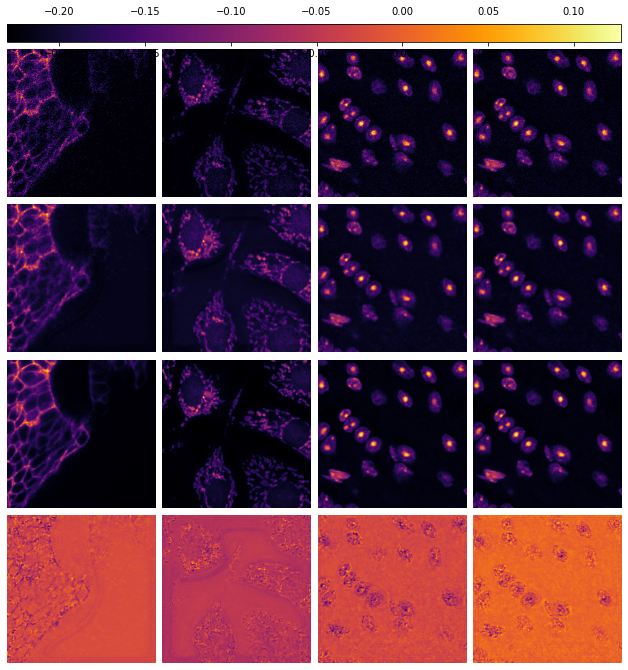
\includegraphics[width=.65\linewidth,valign=t]{my_folder/images/denoising/fix_test_epoch_50.png}
	\end{subfigure}
	\hfill %выровнять по ширине
	\adjustbox{minipage=1.3em,valign=t}{\subcaption{}\label{fig:train-iters-b}}%
	\begin{subfigure}[t]{\dimexpr.5\linewidth-1.3em\relax}
		\centering
		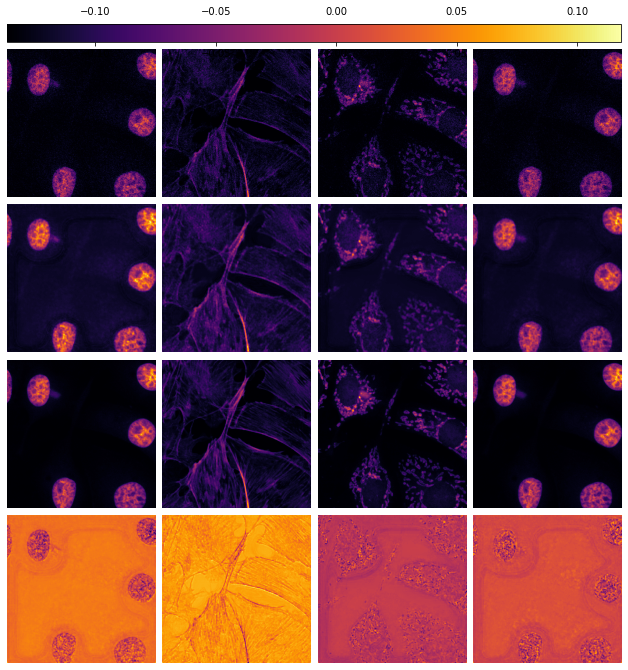
\includegraphics[width=.65\linewidth,valign=t]{my_folder/images/denoising/fix_test2_epoch_50.png}
	\end{subfigure}
	\\[20pt]
	\captionsetup{justification=centering} %центрировать
	\caption{Визуальный анализ на 50 эпохе, содержащий несколько тестовых изображений (слева-направо), а также этапы денойзинга (сверху-вниз): чистое изображение, зашумлённое, обесшумленное, разница между обесшумленным и чистым: {\itshape a} --- тест из 1-ых 4-ёх изображений; {\itshape b} --- тест из 2-ых 4-ёх изображений} 
	\label{fig:train-iters}
\end{figure}

\textbf{Итоговые результаты}.
В конце обучения были построены графики сходимости метрики PSNR и RMSE. Оценки показали высокую точность предсказаний \firef{fig:denoising-training-metrics}.

\begin{figure}[H]
	\adjustbox{minipage=1.3em,valign=t}{\subcaption{}\label{fig:denoise-train-a}}%
	\begin{subfigure}[t]{\dimexpr.5\linewidth-1.3em\relax}
		\centering
		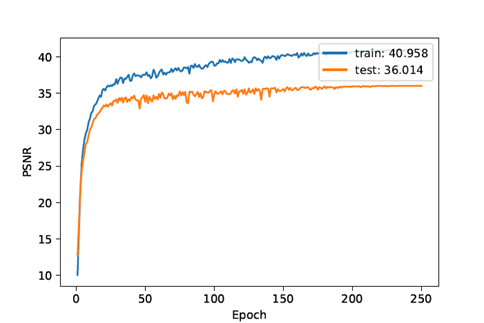
\includegraphics[width=.95\linewidth,valign=t]{my_folder/images/denoising/psnr_training.png}
	\end{subfigure}
	\hfill %выровнять по ширине
	\adjustbox{minipage=1.3em,valign=t}{\subcaption{}\label{fig:denoise-train-b}}%
	\begin{subfigure}[t]{\dimexpr.5\linewidth-1.3em\relax}
		\centering
		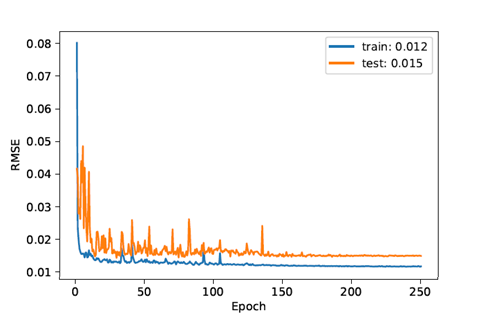
\includegraphics[width=.95\linewidth,valign=t]{my_folder/images/denoising/rmse_training.png}
	\end{subfigure}
	\\[20pt]
	\captionsetup{justification=centering} %центрировать
	\caption{Графики, отображающие метрии PSNR и RMSE в процессе обучения на протяжении всех 200 эпох. Синий график - результаты на тренировочной выборке; оранжевый - результаты на валидационной выборке: {\itshape a} --- метрика PSNR; {\itshape b} --- метрика RMSE} 
	\label{fig:denoising-training-metrics}
\end{figure}

\subsection{Эксперементы денойзинга}
\par В этом подпараграфе будет рассмотрен подробный анализ работы алгоритма 3D денойзинга с использованием различных методов, как нейросети Noise2Noise, нелокального фильтра Non-local means, так и их комбинаций. Оценка будет производиться с помощью описанных ранее метрик. 
\par Измерение времени работы методов денойзинга проводилось на центральном процессоре (CPU) Intel Xeon Gold 6230 и 64 Gb RAM, предоставленном также от Yandex DataSphere. 
\subsubsection{Оценка метрик алгоритма 3D денойзинга}
\par Первым экспериментом работы методов стало обесшумливание синтетического изображения трубочек размером 7x2048x2048, на который накладывался различный шум Пуассона с параметром $\lambda \in [1, 2, 4, 8, 16]$.
\par Сначала рассмотрим результаты работы методов для уровня шума $\lambda=16$. На \firef{fig:synthetic-denoise-16} можно увидеть, что все методы справляются с задачей денойзинга, особенно касаемо областей, где нет объекта(фон). Также можно заметить, что нелокальный фильтр и соответствующая комбинация фильтр+сеть удаляет части объекта с низкой интенсивностью. Напротив методы Noise2Noise и комбинация сеть+фильтр лучше сохраняют детали изображения.  
\begin{minipage}{\textwidth}
	\centering
	\vspace{\mfloatsep} % интервал  	
	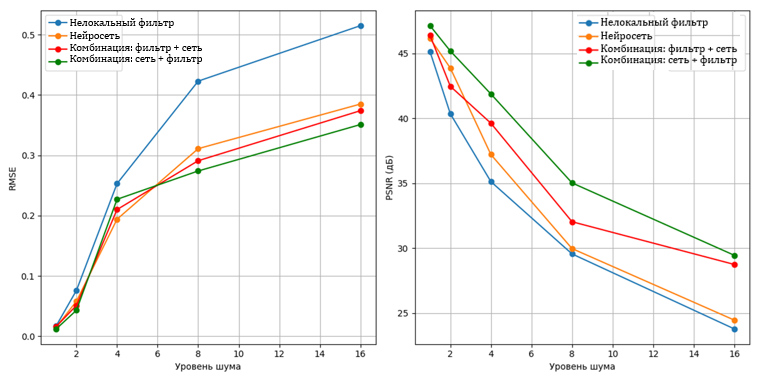
\includegraphics[keepaspectratio=true,scale=0.67] {my_folder/images/denoising/metrics_noise.png}
	\captionof{figure}{Визуальный анализ на синтетических данных для $\lambda=16$}
	\label{fig:synthetic-denoise-16}  
	\vspace{\mfloatsep} % интервал  	
\end{minipage}
\par Однако более информативными будут значения, приведённые в таблице \ref{tab:synthetic-denoise-16}. Из них можно сделать следующие выводы:
\begin{enumerate}
	\item Нелокальный фильтр (NLM) демонстрирует наименьшее время работы, но при этом имеет наибольшие значения RMSE и наименьшие значения PSNR среди всех рассмотренных методов.
	\item Нейросеть (N2N) требует больше времени на обработку, но достигает лучших результатов по сравнению с нелокальным фильтром как по RMSE, так и по PSNR.
	\item Комбинированные методы (фильтр+сеть и сеть+фильтр) показывают лучшие показатели по метрикам RMSE и PSNR в сравнении с нейросетевым подходом. При этом комбинация "сеть+фильтр" демонстрирует наилучшие результаты, чем "фильтр+сеть", как и в случае визуального анализа.
\end{enumerate}  
\begin{table} [H]% Пример оформления таблицы
	\centering\small
	\caption{Численный анализ на синтетических данных для $\lambda=16$}%
	\label{tab:synthetic-denoise-16}
	\begin{tabular}{|l|l|l|l|}
		\hline
		Методы&Время работы, с&RMSE&PSNR, дБ\\
		\hline
		Нелокальный фильтр, NLM
		&15&0.51&23.8\\ \hline
		Нейросеть, N2N&72&0.38&24.5\\ \hline
		Комбинация фильтр+сеть
		&87&0.37&28.7\\ \hline Комбинация сеть+фильтр
		&88&0.35&29.5\\ \hline		
	\end{tabular}
	\normalsize% возвращаем шрифт к нормальному
\end{table}
\par Также был проведён анализ работы методов в зависимости от уровня шума $\lambda \in [1, 2, 4, 8, 16]$. На \firef{fig:synthetic-denoise-16-all} можно увидеть, что лучшими по обоим показателям оказались комбинированные методы, а также что с увеличением уровня шума RMSE всех методов увеличивается, а PSNR соответственно уменьшается. Наименьшие значения RMSE и наибольшие значения PSNR достигаются при комбинации методов "сеть+фильтр", что свидетельствует о большей устойчивости этого подхода к высоким уровням шума.
\begin{minipage}{\textwidth}
	\centering
	\vspace{\mfloatsep} % интервал  	
	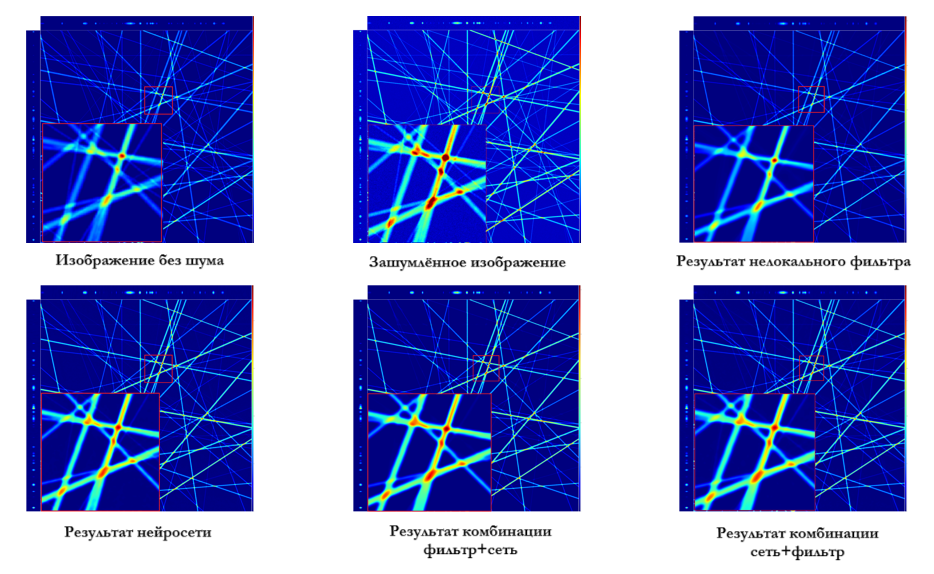
\includegraphics[keepaspectratio=true,scale=0.67] {my_folder/images/denoising/test_16_all.png}
	\captionof{figure}{Численный анализ на синтетических данных в зависимости от уровня шума $\lambda$}
	\label{fig:synthetic-denoise-16-all}  
	\vspace{\mfloatsep} % интервал  	
\end{minipage}
\par Таким образом, комбинированные подходы обеспечивают наилучшее качество денойзинга, несмотря на большее время обработки, что делает их предпочтительными для задач, где качество результата критично.
\subsubsection{Денойзинг реальных данных}
\par Для проверки работоспособности методов были проведены эксперименты по денойзингу на реальных данных. В этих экспериментах не будут представлены результаты метрик PSNR и RMSE, так как отсутствует точное изображение, с которым можно было бы сравнить обработанные данные.
\par  Помимо этого, был проведен анализ сегмента реального изображения, на котором отсутствует объект. Этот анализ включает вычисление основных статистических характеристик распределения, таких как среднее, дисперсия и среднеквадратическое отклонение (СКО). Проведение статистического анализа для области, содержащей фон, необходимо по нескольким причинам:
\begin{itemize}[]
	\item Оценка работоспособности методов денойзинга по удалению шумов на реальных снимках.
	\item Исследование природы шума и подтверждение его распределения по Пуассону.
\end{itemize}
\par Начнём с эксперимента на изображении трубочек размером 40x200x200. На \firef{fig:real-segment} приведены результаты денойзинга. На основании данных результатов можно сделать следующие выводы:
\begin{enumerate}[]
	\item Нелокальный фильтр справляется хорошо с шумами низкой интенсивности, однако сам объект остался в зашумлённом состоянии.
	\item Нейросеть успешно обесшумила весь снимок, сделав объект более чётким и очерченным.
	\item Комбинированные методы совместили достоинства обоих подходов. Интенсивности шумов на фоне изображения (где нет объекта) значительно уменьшились, что свидетельствует о высокой эффективности методов в удалении шумов. При этом комбинация "сеть + фильтр" лучше сглаживает шумы и сохраняет детали объекта по сравнению с комбинацией "фильтр + сеть".
\end{enumerate}
\par Также были посчитаны основные случайные величины в фоновом сегменте на данном снимке. Из полученных результатов в таблице  \ref{tab:real-segment} можно сделать следующие выводы:
\begin{enumerate}[]
	\item Добавочный шум на реальных снимках распределён по Пуассону, так как среднее и дисперсия практически  равны ($M[x] \approx D[x] = \lambda$, где $\lambda$ - возможный уровень шума)
	\item Нелокальный фильтр и нейросеть справляются с задачей, так как все измеряемые статистические величины уменьшаются.
	\item Комбинированные методы показывают улучшенные результаты: среднее значение интенсивности шума уменьшается более чем в 2 раза, а дисперсия уменьшается в 1.5 раза.
\end{enumerate}
\begin{minipage}{\textwidth}
	\centering
	\vspace{\mfloatsep} % интервал  	
	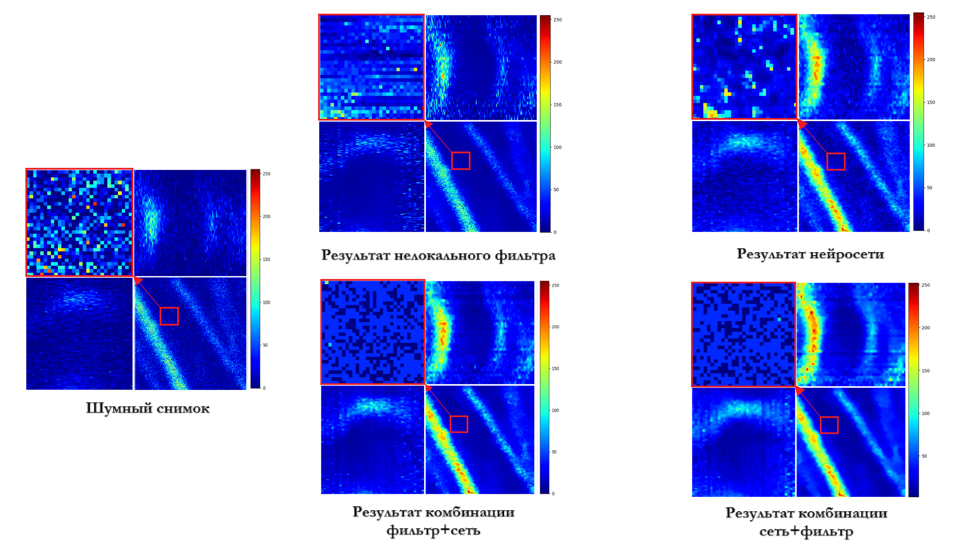
\includegraphics[keepaspectratio=true,scale=0.67] {my_folder/images/denoising/real_colors.png}
	\captionof{figure}{Денойзинг реального снимка; Сегмент, не содержащий объекта}
	\label{fig:real-segment}  
	\vspace{\mfloatsep} % интервал  	
\end{minipage}
\begin{table} [H]% Пример оформления таблицы
	\centering\small
	\caption{Статистика интенсивности шума на реальном снимке}%
	\label{tab:real-segment}		
	\begin{tabular}{|l|l|l|l|}
		\hline
		Методы&Среднее&Дисперсия&СКО\\
		\hline	
		Шумный снимок
		&8.3&8.4&2.9\\ \hline
		Нелокальный фильтр, NLM
		&6&3.1&1.6\\ \hline
		Нейросеть, N2N&5.5&3.3&1.8\\ \hline
		Фильтр+сеть
		&2.3&2.7&1.6\\ \hline Сеть+фильтр
		&2.2&2.8&1.7\\ \hline			
	\end{tabular}
	\normalsize% возвращаем шрифт к нормальному
\end{table}
\par Также для реальных снимков разных размеров были построены графики интенсивностей вдоль линии, отмеченной красной линией. На основе \firef{fig:intensity-test1-a} и табл. \ref{tab:intensity-test1} можно сказать, что:
\begin{enumerate}[]
	\item Время работы нелокального фильтра и нейросети практически не отличается из-за небольшого размера изображения.
	\item Нейросеть лучше подавляет пики интенсивностей, чем нелокальный фильтр.
	\item Комбинация "сеть+фильтр" даёт наиболее гладкий график интенсивностей, что указывает на более эффективное устранение шумов и сохранение деталей.
\end{enumerate}
\begin{figure}[H]
	\adjustbox{minipage=1.3em,valign=t}{\subcaption{}\label{fig:intensity-test1-a}}%
	\begin{subfigure}[t]{0.6\textwidth\relax}
		\centering
		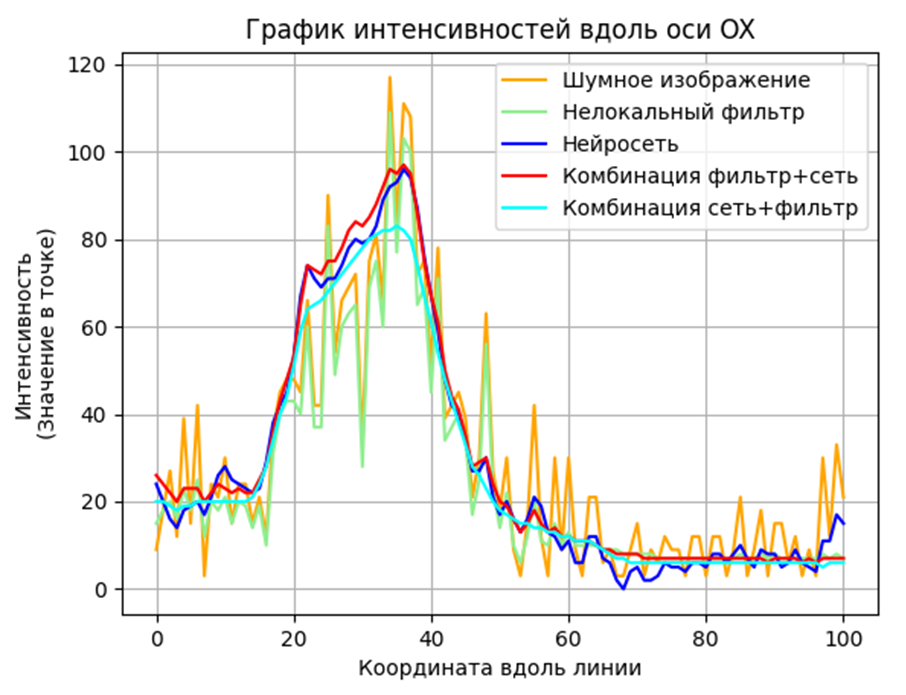
\includegraphics[width=.95\linewidth,valign=t]{my_folder/images/denoising/intensity_test1.png}
	\end{subfigure}
	\hfill %выровнять по ширине
	\adjustbox{minipage=1.3em,valign=t}{\subcaption{}\label{fig:denoise-train-b}}%
	\begin{subfigure}[t]{0.3\textwidth\relax}
		\centering
		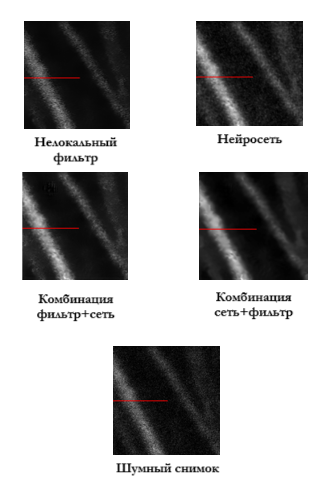
\includegraphics[width=.95\linewidth,valign=t]{my_folder/images/denoising/intensity_test1_images.png}
	\end{subfigure}
	\\[20pt]
	\captionsetup{justification=centering} %центрировать
	\caption{График интенсивностей вдоль оси OX для реального изображения размером 40x200x200: {\itshape a} --- График интенсивностей вдоль оси OX; {\itshape b} --- Результаты денойзинга} 
	\label{fig:intensity-test1}
\end{figure}
\begin{table} [H]% Пример оформления таблицы
	\centering\small
	\caption{Статистика интенсивности шума на реальном снимке}%
	\label{tab:intensity-test1}		
	\begin{tabular}{|l|l|l|l|l|}
		\hline
		 &Нелокальный фильтр&Нейросеть&Фильтр+сеть&Сеть+фильтр\\
		\hline	
		Время, cек.
		&1.5&1.5&3.1&3.2\\ \hline
	\end{tabular}
	\normalsize% возвращаем шрифт к нормальному
\end{table}
\par Для снимка большой размерности (29x2048x2048) были также применены различные методы денойзинга. Аналогично, для наглядности, построен график интенсивностей \firef{fig:intensity-test2-a}, проходящий сквозь объект снимка. Также было замерено время и записано в \ref{tab:intensity-test2}. Итак, можно заметить следующее: 
\begin{enumerate}[]
	\item  Нелокальный фильтр (NLM) работает значительно быстрее, чем нейросеть и комбинированные методы, но результат денойзинга значительно хуже.
	\item Нейросеть работает дольше, но даёт график интенсивностей с меньшим числом перепадов интенсивностей.
	\item График интенсивностей комбинированных методов показывает, что комбинации дают более гладкий результат, чем отдельно взятые методы, что свидетельствует о лучшем сохранении деталей и снижении шумов.
	\item Из двух комбинаций метод сеть+фильтр дает наиболее гладкий график интенсивностей и лучше сохраняет детали изображения.
\end{enumerate}
\begin{figure}[H]
	\adjustbox{minipage=1.3em,valign=t}{\subcaption{}\label{fig:intensity-test2-a}}%
	\begin{subfigure}[t]{0.6\textwidth\relax}
		\centering
		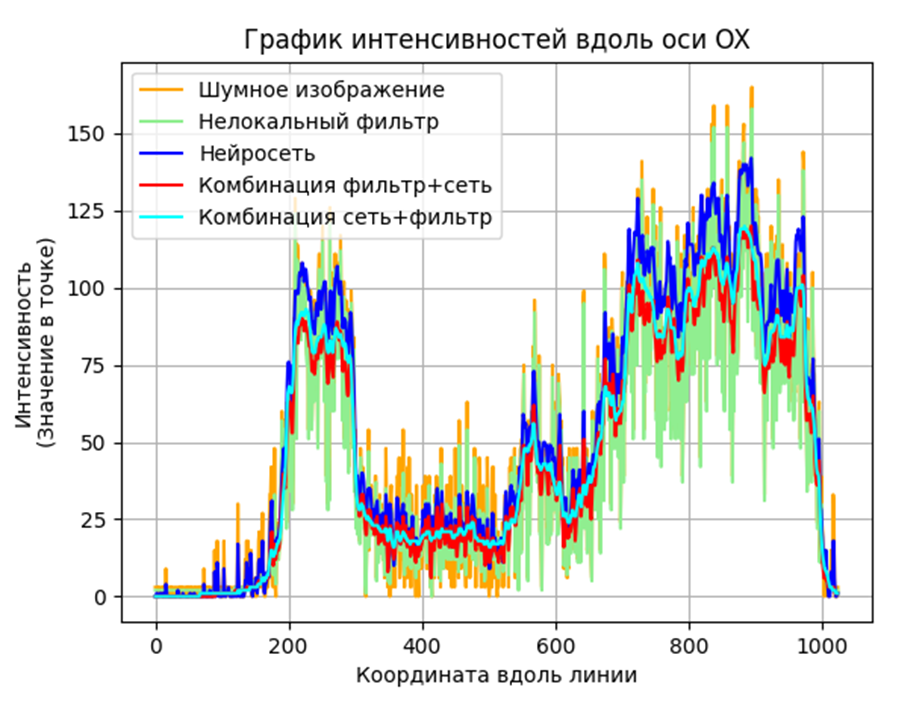
\includegraphics[width=.95\linewidth,valign=t]{my_folder/images/denoising/intensity_test2.png}
	\end{subfigure}
	\hfill %выровнять по ширине
	\adjustbox{minipage=1.3em,valign=t}{\subcaption{}\label{fig:intensity-test2-b}}%
	\begin{subfigure}[t]{0.3\textwidth\relax}
		\centering
		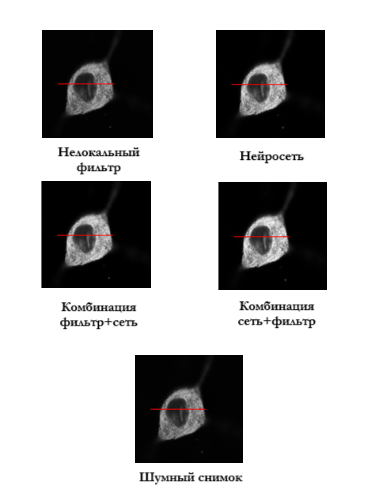
\includegraphics[width=.95\linewidth,valign=t]{my_folder/images/denoising/intensity_test2_images.png}
	\end{subfigure}
	\\[20pt]
	\captionsetup{justification=centering} %центрировать
	\caption{График интенсивностей вдоль оси OX для реального изображения размером 29x2048x2048: {\itshape a} --- График интенсивностей вдоль оси OX; {\itshape b} --- Результаты денойзинга} 
	\label{fig:intensity-test2}
\end{figure}
\begin{table} [H]% Пример оформления таблицы
	\centering\small
	\caption{Статистика интенсивности шума на реальном снимке}%
	\label{tab:intensity-test2}		
	\begin{tabular}{|l|l|l|l|l|}
		\hline
		&Нелокальный фильтр&Нейросеть&Фильтр+сеть&Сеть+фильтр\\
		\hline	
		Время
		&51 сек.&4.6 мин.&5.1 мин.&5.2 мин.\\ \hline
	\end{tabular}
	\normalsize% возвращаем шрифт к нормальному
\end{table}

\section{Результаты автоматической сегментации}
\par Результаты показывают, что алгоритм автоматической сегментации сфер имеет значительное преимущество перед ручной сегментацией. На примере изображения размером \textbf{36x2048x2048} время выполнения для автосегментации составило всего \textbf{0.83 секунды} с усреднением и 0.78 секунды без усреднения, в то время как \textbf{ручная сегментация} занимает значительно больше времени, около \textbf{10-15 минут}. Эксперименты для 2-ух сегментаций проводились на CPU: \textbf{AMD Ryzen 7 5700U with Radeon Graphics 1.80 GHz}.

\par На \firef{fig:autosegm-res} приведено визуальное представление результата автосегментации:\\
\noindent % for correct centering
\begin{minipage}{\textwidth}
	\centering
	\vspace{\mfloatsep} % интервал  	
	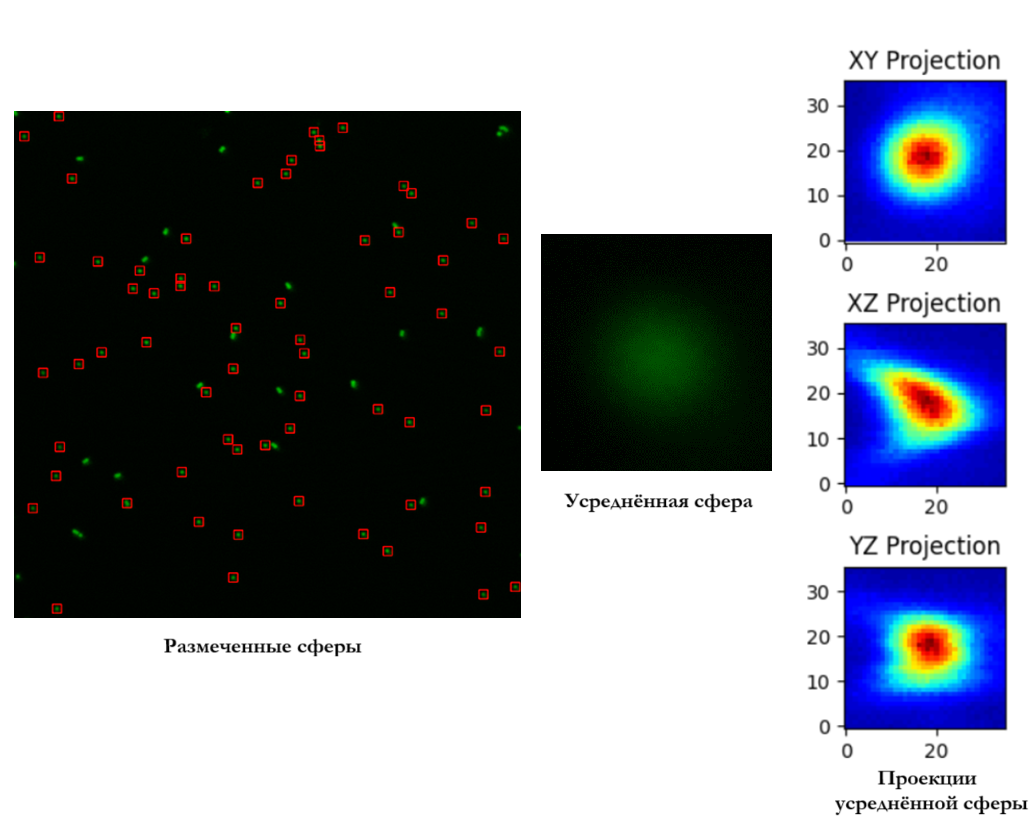
\includegraphics[keepaspectratio=true,scale=0.37] {my_folder/images/autosegm/autosegm_res.png}
	\captionof{figure}{Результат автоматической сегментации сфер}\label{fig:autosegm-res}  
	\vspace{\mfloatsep} % интервал  	
\end{minipage}

\par Применение денойзинга значительно улучшает качество изображений.  На \firef{fig:autosegm-res-denoise} можно увидеть, что предварительно обработанное изображение со сферами нейронной сетью Noise2Noise, после процесса сегментации и усреднения даёт более округлую и отчётливую усреднённую сферу. 
\begin{minipage}{\textwidth}
	\centering
	\vspace{\mfloatsep} % интервал  	
	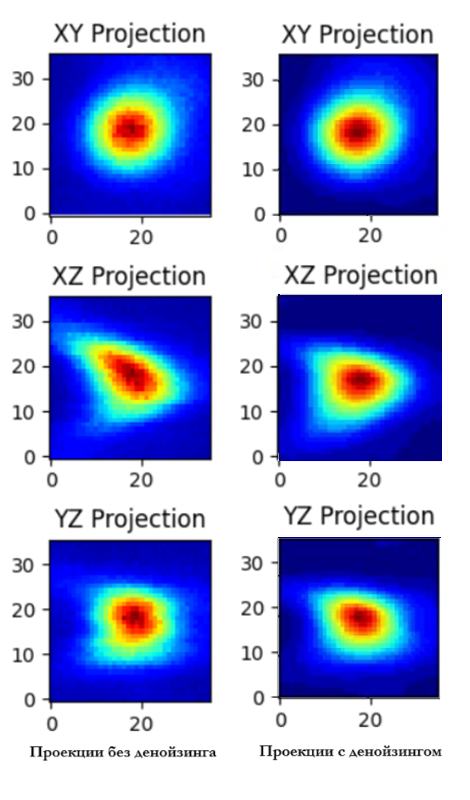
\includegraphics[keepaspectratio=true,scale=0.57] {my_folder/images/autosegm/autosegm_res_denoised.png}
	\captionof{figure}{Сравнение результатов сегментации сфер с и без денойзинга}\label{fig:autosegm-res-denoise}  
	\vspace{\mfloatsep} % интервал  	
\end{minipage}

\par Всё выше перечисленное говорит о том, что использование автоматической сегментации сфер оправдано, особенно учитывая сложность и время, затрачиваемое на ручную сегментацию при большом количестве сфер на изображении. Применение предварительного денойзинга дополнительно улучшает точность и качество сегментации, что делает этот подход еще более полезным для обработки изображений с высоким уровнем шума. 

\section{Описание архитектуры онлайн-сервиса деконволюции}
\par Результат проделанной работы был оформлен в виде онлайн-сервиса с встроенными процессами обработки изображений с помощью языков программирования Python и JavaScript. Архитектура сервиса включает следующие технологии и инструменты: Django, ReactJS, Docker, Redis, Nginx, Celery, Flower.
\par Все процессы улучшения изображений могут быть представлены в виде идущими друг за другом шагами обработки: например, загрузка изображений, настройка параметров, обработка, сохранение и визуализация результатов. Потому веб-интерфейс каждой отдельной функциональности представляемого ПО реализован в виде степпера (от англ. step - шаги). Данный степпер даёт возможность пользователю наблюдать  промежуточные результаты на каждом шаге обработки данных, а также на этапах до и после обработки. Кроме того в переходах между разными этапами (степперами) результаты на предыдущем шаге сохраняются в кэше (высокоскоростной памяти небольшого размера), чтобы минимизировать задержки при доступе к данным. 
\par Архитектура серверной части поддерживает масштабируемость, гибкость, высокую производительность, мониторинг и логгирование, а также сервис является надёжным и простым в использовании благодаря контейнеризации Docker. Также сервис обладает модульностью - возможностью интеграции с ПО лаборатории и загрузки изображений в базу данных (БД).
\par Итак, перейдём к рассмотрению конкретных этапов обработки изображений:
\begin{enumerate}[]
	\item \textit{Сегментация (извлечение) флуоресцентных сфер}:\\
	На данном этапе (см. \firef{fig:bead-stepper}) пользователь может гибко комбинировать два подхода к сегментации: ручной и автоматический. Настройка параметров и использование слайдеров значительно упрощает процесс извлечения образцов для пользователя.\\
	\begin{minipage}{\textwidth}
		\centering
		\vspace{\mfloatsep} % интервал  	
		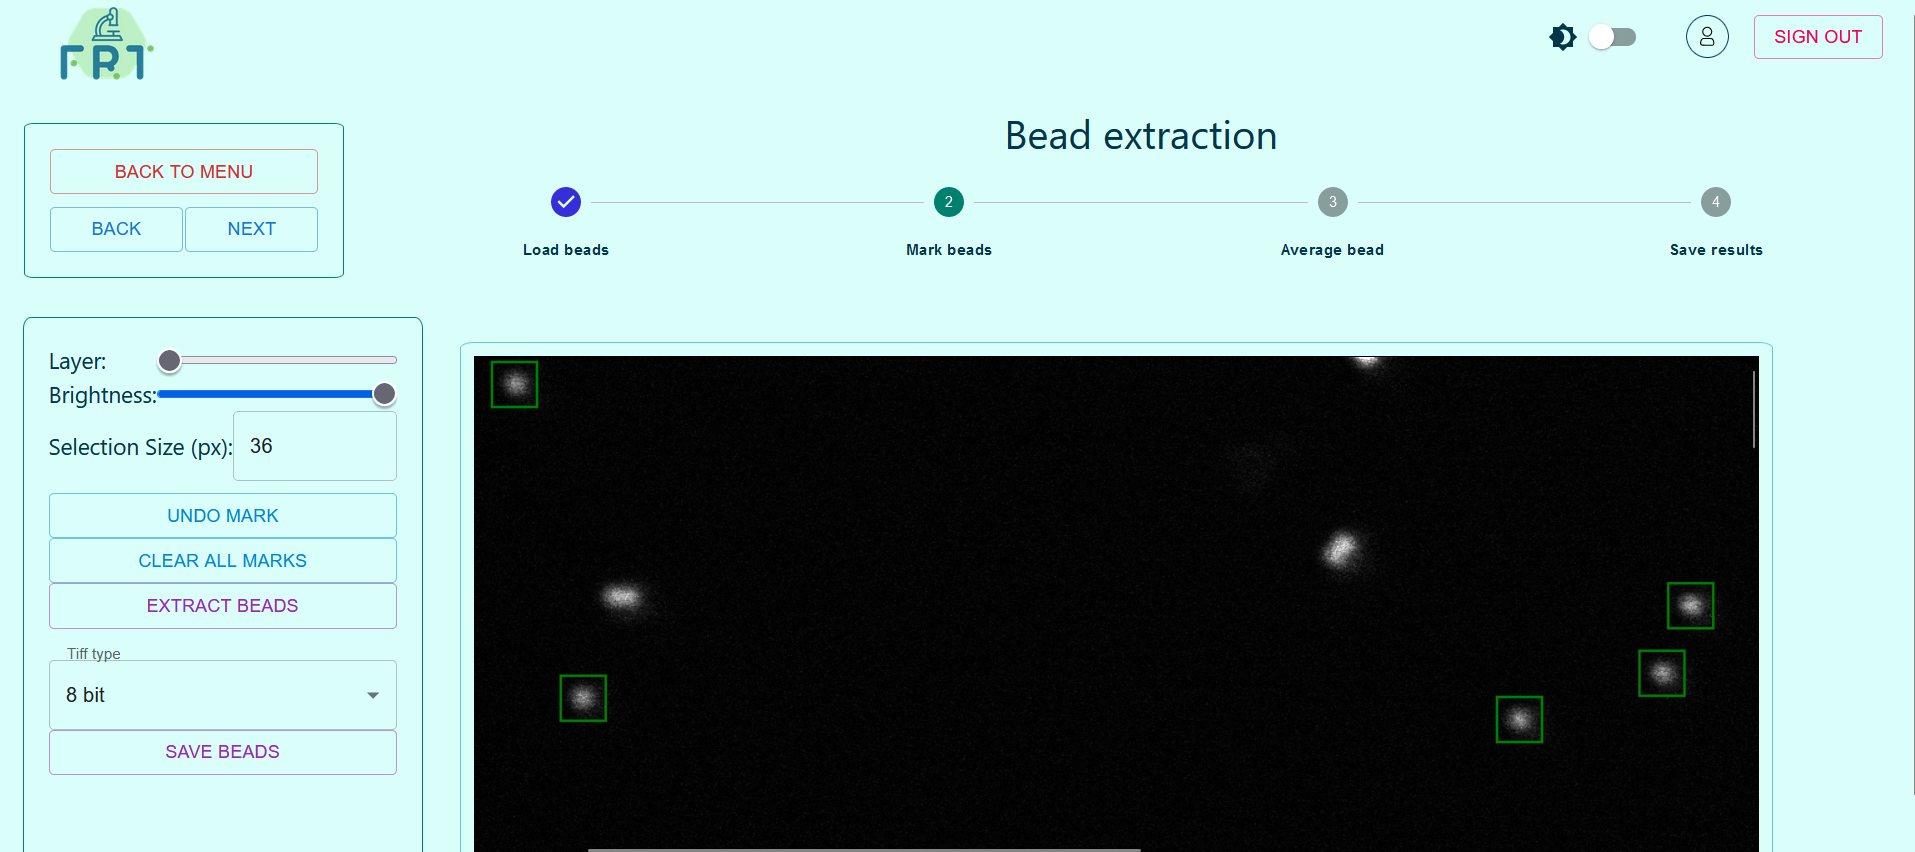
\includegraphics[keepaspectratio=true,scale=0.25] {my_folder/images/online_service/steper_extractor.png}
		\captionof{figure}{Процесс сегментации сфер}\label{fig:bead-stepper}  
		\vspace{\mfloatsep} % интервал  	
	\end{minipage}
\item \textit{Усреднение сфер}:\\
На данном этапе (см. \firef{fig:avg-stepper}) есть возможность просмотра выбранных сфер, их усреднение с выбором метода предобработки.\\
\begin{minipage}{\textwidth}
	\centering
	\vspace{\mfloatsep} % интервал  	
	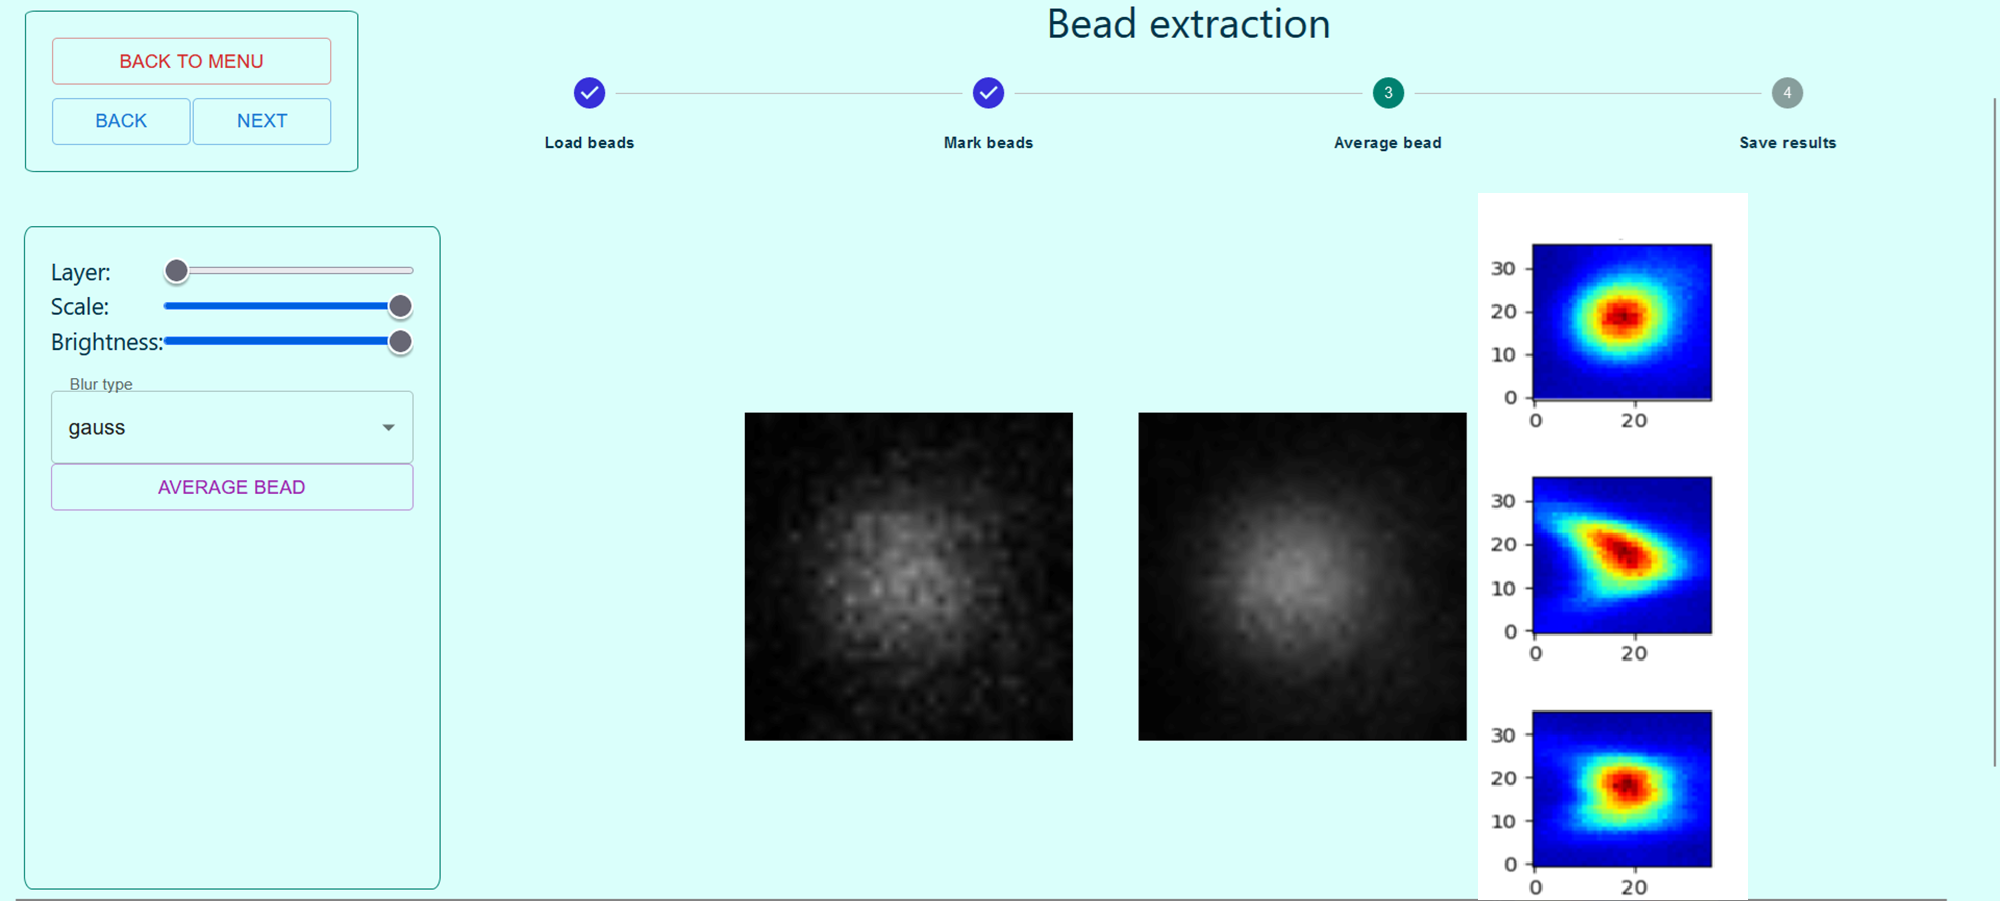
\includegraphics[keepaspectratio=true,scale=0.25] {my_folder/images/online_service/averaging_bead.png}
	\captionof{figure}{Процесс усреднения трёхмерных сфер}\label{fig:avg-stepper}  
	\vspace{\mfloatsep} % интервал  	
\end{minipage}
\item \textit{Вычисление Функции рассеяния точки (ФРТ)}:\\
На 2-ой степпер (см. \firef{fig:psf-stepper}) предзагружается усреднённая сфера и пользователь можеть получить ФРТ эксперементальным способом, применяя метод деконволюции, меняя различные гиперпараметры: размер сферы, число иттераций, параметр регуляризации и вид метода Ричардсона-Люси (РЛ).\\
\begin{minipage}{\textwidth}
	\centering
	\vspace{\mfloatsep} % интервал  	
	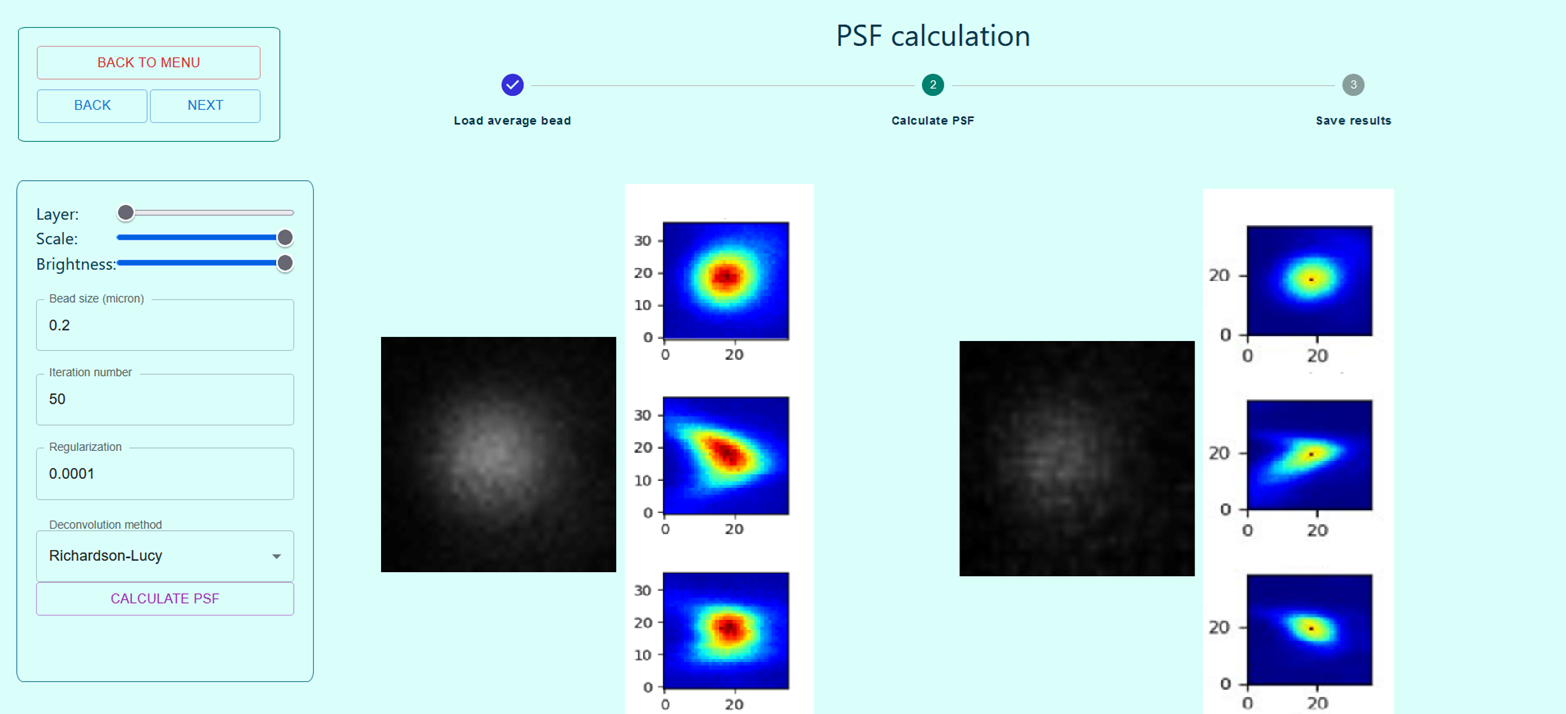
\includegraphics[keepaspectratio=true,scale=0.3] {my_folder/images/online_service/stepper_psf.png}
	\captionof{figure}{Процесс вычисления ФРТ}\label{fig:psf-stepper}  
	\vspace{\mfloatsep} % интервал  	
\end{minipage}
\item \textit{Деконволюция трёхмерного изображения}:\\
В последнем степпере (см. ) загружается эФРТ и в интерактивном формате, аналогично вычислению ФРТ, пользователь может обработать трёхмерное изображение в реальном времени. Как можно увидеть на \firef{fig:deconv-stepper}, что результат деконволюции сделал сферы более отчётливыми и отделимыми друг от друга. \\
\begin{minipage}{\textwidth}
	\centering
	\vspace{\mfloatsep} % интервал  	
	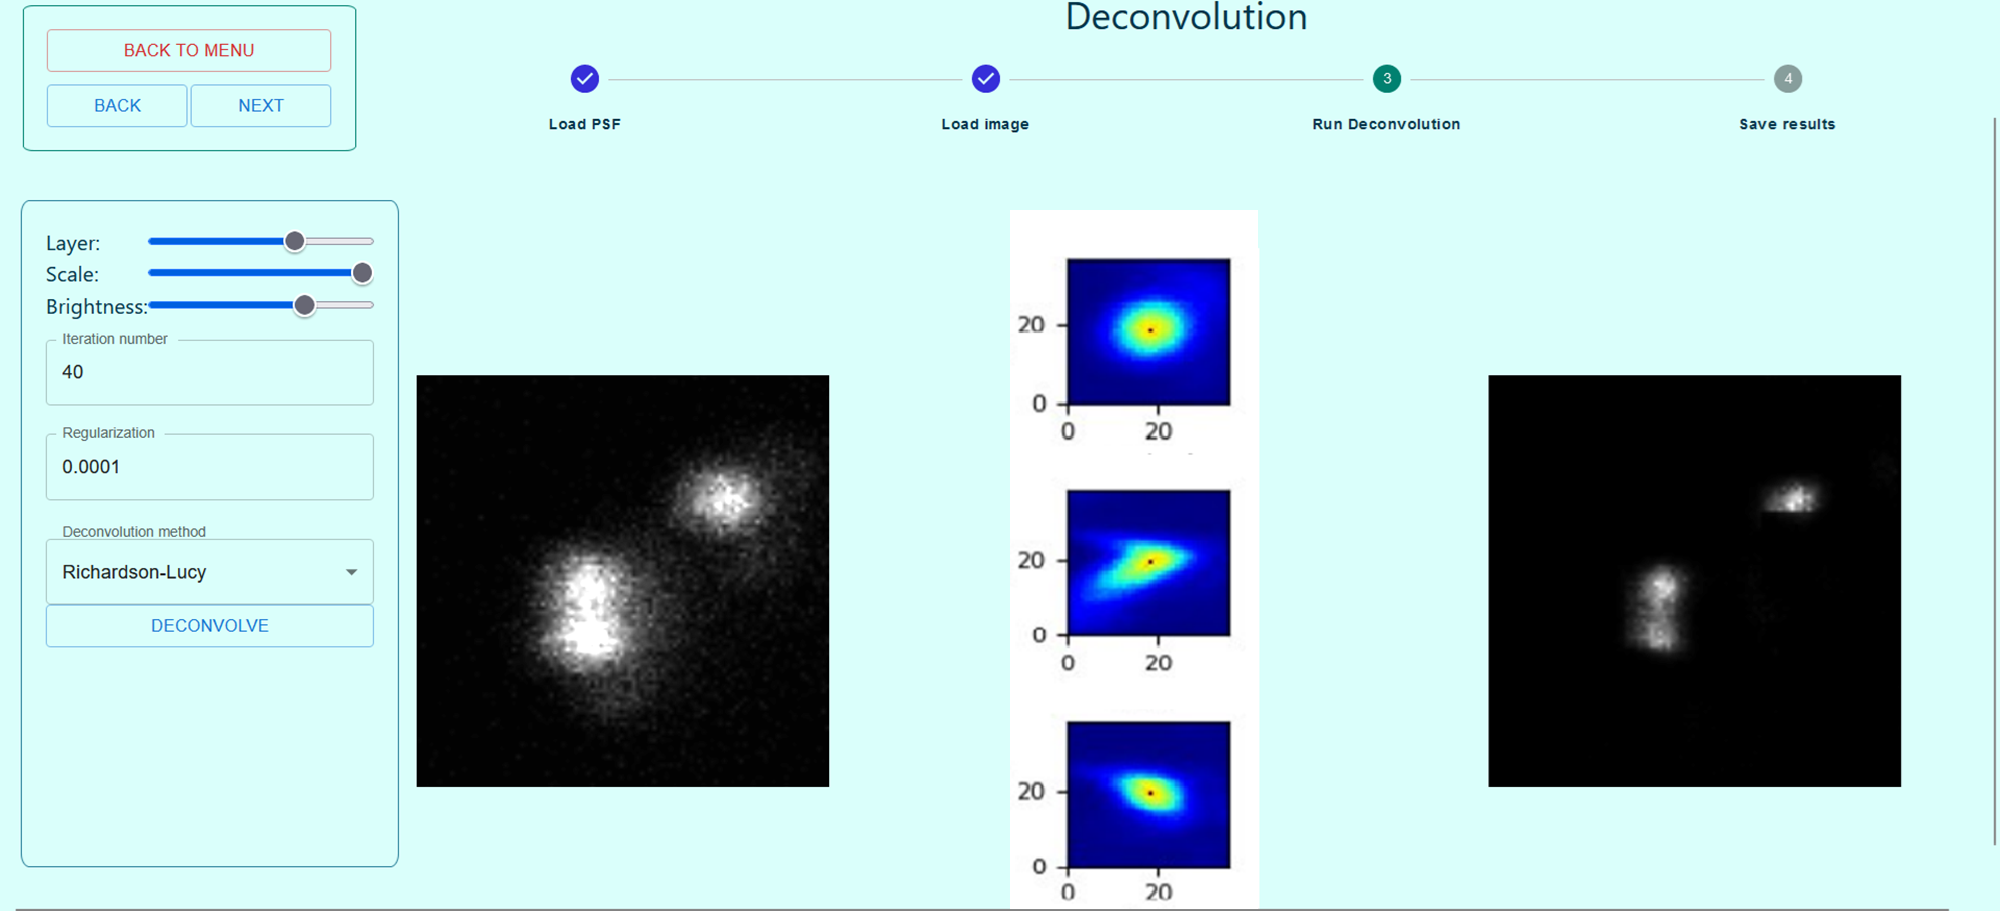
\includegraphics[keepaspectratio=true,scale=0.25] {my_folder/images/online_service/deconvolution.png}
	\captionof{figure}{Процесс деконволюции изображений}\label{fig:deconv-stepper} 
	\vspace{\mfloatsep} % интервал  	
\end{minipage}
\end{enumerate}

% не рекомендуется использовать отдельную section <<введение>> после лета 2020 года
%\section{Введение} \label{ch3:intro}


%% Вспомогательные команды - Additional commands
%
%\newpage % принудительное начало с новой страницы, использовать только в конце раздела
%\clearpage % осуществляется пакетом <<placeins>> в пределах секций
%\newpage\leavevmode\thispagestyle{empty}\newpage % 100 % начало новой страницы